\section{Berry curvature in Gapped graphene}

The Hamiltonian for the gapped graphene near the point $K_1$ and $K_2$ can be written as 
\begin{equation}
    H_{K_1}=-H_{K_2}^\dagger=
    \begin{bmatrix}
        \Delta & \hbar v_F(k_x+ik_y)\\
        \hbar v_f(k_x-ik_y)& -\Delta
    \end{bmatrix}
\end{equation}
Where $\Delta$ is the energy gap and $v_F$ is the Fermi velocity. For ease of notation we are going to work with just $H_{K_1}$ and drop the $K_1$,\footnote{Don't worry, I'll bring it back if when we'll need it} and for ease of computation we define $\vect q=\hbar v_F\vect k$
\begin{equation}
    H=
    \begin{bmatrix}
        \Delta & q_x+iq_y\\
        q_x-iq_y& -\Delta
    \end{bmatrix}=
    \sigma_x q_x + \sigma_y q_y + \sigma_z \Delta \equiv  \boldsymbol \sigma \cdot \vect E
\end{equation}

Here the enegry vector $\vect E$ is defined as $\vect E =( q_x,q_y,\Delta)$. The nice things about it is that $E=|\vect E|=\sqrt{q_x^2+q_y^2+\Delta^2}$ is the positive eigenvalue of the hamiltonian (the negative eigenvalue is just $-E$).\newline
To calculate the Berry curvature we are first going to calculate the Berry connection \ref{eq:connection}, and to calultate the Berry connection we need the eigenvectors which are well known for the Hamiltonian of the form $\boldsymbol \sigma \cdot \vect{E}$.

\begin{equation}
    \ket{+;\theta,\phi}=
    \begin{bmatrix}
        \cos{\frac \theta 2}\\
        e^{i\phi}\sin{\frac \theta 2}
    \end{bmatrix}
    \quad
    \ket{-;\theta,\phi}=
    \begin{bmatrix}
        -e^{-i\phi}\sin{\frac \theta 2}\\
        \cos{\frac \theta 2}
    \end{bmatrix}
\end{equation}
Where $\theta$ and $\phi$ are the coordinates of $\vect E$ in the polar representation

Now we can calculate the Berry connection

\begin{equation}
    A_\theta^+=-A_\theta^-=0 \quad A_\phi^+=-A_\phi^-=\sin^2\frac \theta 2
\end{equation}

This means that the Berry curvature is
\begin{equation}
    \Omega^+_{\theta\phi}=-\Omega^-_{\theta\phi}=\partial_\theta A^+_\phi=\frac{\sin \theta}2
\end{equation}

From now on we are going to work with $\Omega^+$ and we are going to drop the $+$ sign to make the notation lighter.

We want to express $\Omega$ in terms of $\vect q$, however it's more convenient to write it in terms fo  $\cos \theta$ and $\phi$, so we do a small coordinate transformation


\begin{equation}
    \Omega_{\theta\phi}=\frac{\partial\cos\theta}{\partial \theta}\Omega_{\cos(\theta)\phi} \rightarrow \Omega_{\cos(\theta)\phi}=\frac 12
\end{equation}



Now we can easily make the transformation to express $\Omega$ in terms of $\vect q$. The Berry curvature transforms like any other tensor under coordinate transformation, so

\begin{equation}
    \Omega_{q_xq_y}=\frac{\partial\cos \theta}{\partial q_x}\frac{\partial \phi}{\partial q_y}\Omega_{\cos(\theta)\phi}+\frac{\partial \phi}{\partial q_x}\frac{\partial\cos \theta}{\partial q_y}\Omega_{\phi\cos(\theta)} 
\end{equation}

That can be rewritten as

\begin{equation}
    \Omega_{q_xq_y}=\frac 12 \det\bigg[\frac{\partial (cos\theta,\phi)}{\partial (q_x,q_y)}\bigg]=\frac 12 \frac{\Delta^2}{q^2E^3}(q_x+q_y-2q)
\end{equation}


And finally we can express it in terms of $\vect k$
\begin{equation}
    \Omega_{k_xk_y}=(\hbar v_F)^2\Omega_{q_xq_y}=\frac {\hbar v_F}2 \frac{\Delta^2}{k^2E^3}(k_x+k_y-2k)
\end{equation}
Up until now we have worked with the Hamiltonian $H_{K_1}$, but with the $K_1$ hidden. The Berry curvature around $K_2$ is equal, but with opposite sign (figure \ref{fig:cones}).\\
\begin{figure}
    \centering
    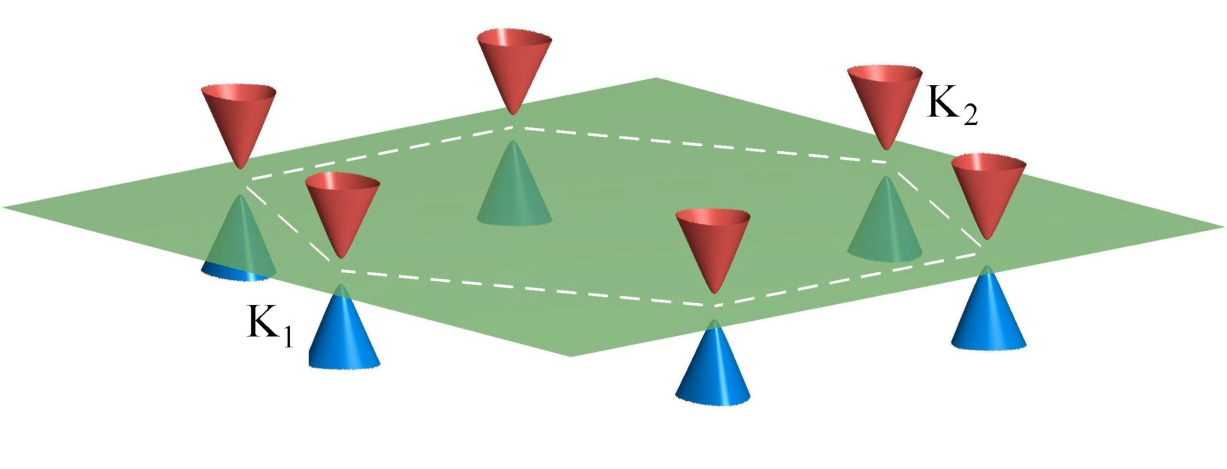
\includegraphics[width=0.7\linewidth]{Immagini/ValleyHall/band_graphene.pdf}
    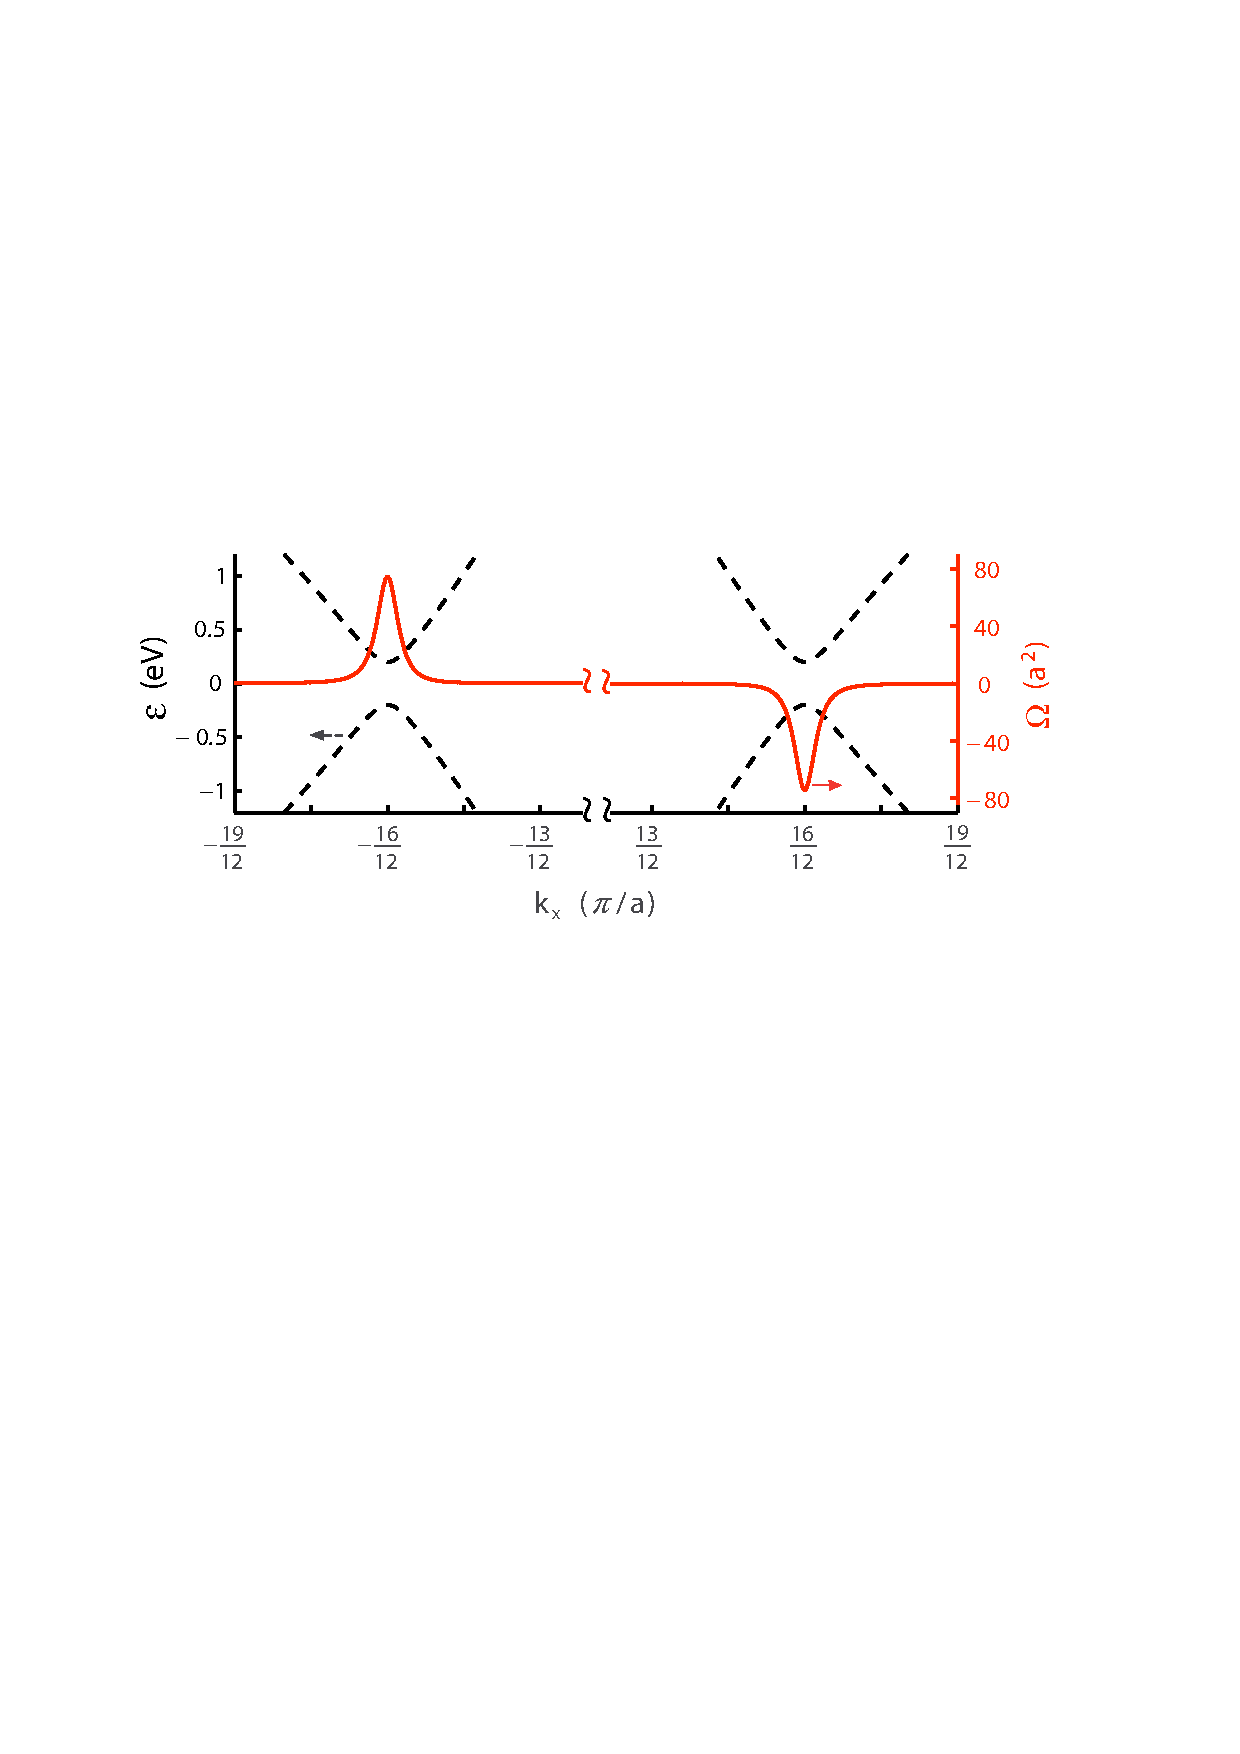
\includegraphics[width=0.7\linewidth]{Immagini/ValleyHall/curvature_graphene.pdf}
    \caption{In the top panel are displayed the Energy bands in 2D. In the bottom panel with the dotted line are displayed a section of the energy bands, and with the continuous red line the Berry curvature.}
    \label{fig:cones}
\end{figure}
Notice how from figure \ref{fig:cones} most of the berry curvature lies near the cones. The nice thing about it is that to calculate the total curvature in any given band, we can calculate the Berry in the two cones, and then sum the results. This is because we know that the total Berry curvature over the band has to be quantized.

Now let's calculate the total Berry curvature in any given cone from equation FINIRE